\documentclass[10pt]{article}

\usepackage[spanish,mexico]{babel}
\usepackage[utf8]{inputenc}
\usepackage{apacite}

\usepackage{anysize}
\marginsize{2cm}{2cm}{2cm}{2cm}
\setlength{\parskip}{8px}

\usepackage{hyperref}

\usepackage{amsmath}
\usepackage{amssymb}
\usepackage{amsfonts}
\usepackage{cancel}

\usepackage{graphicx}
\usepackage{float}

\usepackage{caption}
\usepackage{subcaption}

\usepackage{xcolor}

\usepackage{fancyhdr}

\usepackage{listings}

\usepackage{longtable}
\usepackage{colortbl}
\usepackage{diagbox}
\usepackage{tabularx}

\usepackage{tcolorbox}


\newcolumntype{L}[1]{>{\hsize=#1\hsize\raggedright\arraybackslash}X}%
\newcolumntype{R}[1]{>{\hsize=#1\hsize\raggedleft\arraybackslash}X}%
\newcolumntype{C}[2]{>{\hsize=#1\hsize\columncolor{#2}\centering\arraybackslash}X}%

\renewcommand{\tabularxcolumn}[1]{m{#1}}

\pagestyle{fancy}
\fancyhf{}
\rhead{3CM19}
\lhead{Computing Selected Topics}
\cfoot{\thepage}
\renewcommand{\footrulewidth}{0.4pt}

\definecolor{blueTitle}{rgb}{0.05,0.31,0.48}
\definecolor{blueSub}{rgb}{0.95,0.97,0.98}
\definecolor{blue}{rgb}{0.4, 0.6, 0.8}

\newcommand{\HRule}{\textcolor{blueTitle}{\rule{\linewidth}{0.5mm}}}

\begin{document}

    \thispagestyle{empty}

    \begin{center}
        \begin{minipage}{0.48\textwidth}
            \begin{flushleft}
                \hspace{1cm}
\includegraphics[width=1.5cm]{ipn.png}
            \end{flushleft}
        \end{minipage}
        \begin{minipage} {0.48\textwidth}
            \begin{flushright}
                
\includegraphics[width=2.7cm]{escom.png}
            \end{flushright}
        \end{minipage}

        \vspace*{-2cm}

        \LARGE
        \textcolor{blueTitle}{\textbf{Instituto Politécnico Nacional\\}}
        \LARGE
        \textcolor{blueTitle}{Escuela Superior de Cómputo}

        \vspace{2cm}
        
        \Large
        \textbf{Computing Selected Topics} \\
        \vspace{.3cm}
        Sistemas Complejos
        \vspace{1.5cm}
        
        \Large
        \textbf{Profesor} \\
        \vspace{.3cm}
        Genaro Juárez Martínez
        \vspace{1cm}
        
        \HRule
        \vspace{.4cm}
        {\textbf{Tarea} \smallskip
        
        Resumen de Notas sobre el Juego de la vida y reglas parecidas}
        \HRule
        \vspace{1.5cm}

        \Large
        \textbf{Alumno} \\
        \vspace{.3cm}
       
        Reyes Rodríguez Enrique Abdiel\\
        \vspace{.3cm}
        \vspace{1cm}

        \Large
        \textbf{Grupo} \\
        \vspace{.3cm}
        3CM19
        \vspace{1cm}

    \end{center}
    
    \newpage
    \tableofcontents
    \newpage
    \section{Resumen}
        	
        La teoria de los autómatas celulares en sus inicios fue influenciada por: \\
        \begin{itemize}
            \item John Von Neumann, precursor de los automatas celulares, constructores universales, auto reproduccion y universalidad
            John Horton Conway, creador del juego de la vida, sistemas de planeadores, universalidad espacial
            \item Stephen Wolfram, por sus avances en los automatas celulares de una dimension, clases, complejidad y lenguajes
            \item Mathew Cook, por la minima universalidad de automatas celulares, regla 110 y los sistemas de etiquetado ciclico
        \end{itemize}

    \begin{figure}[h!]
        \centering
        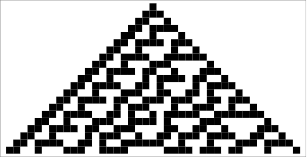
\includegraphics[width=0.5\textwidth]{ac.png}
    \end{figure}
Algunos avances de el juego de la vida fueron
    \begin{itemize}
        \item Una maquina de registros (1982)
        \item Una simulacion de una maquina de Turing (2002)
        \item Conjunto completo de funciones logicas (2003)
        \item Diseño de un constructor universal (2009)
    \end{itemize}


Algo que Conway se preguntaba es si la vida crece indefinidamente, y si el universo se expande por siempre. Hay ciertos patrones que crecen infinitamente como el patron acorn hecho de 7 celulas con una estabilidad en 5206 pasos. 

El primer Jardin del eden, fue encontrado por Roger Banks en 1971, fue requerido de un gran poder computacional en busca de todos los posibles patrones predecesores.

Algunos de los softwares utiles para la representación evolutiva de el juego de la vida es ddlab, Tresvita, Golly

Harold V. McIntosh establece que el automata celular que produce la regla 22 es la proyección en una dimensión de el juego de la vida.

David Artur Eppstein creó una base de datos interactiva donde se pueden ver muchos patrones complejos como guns, gliders, oscillators, etc.\\ \\
Algunas reglas parecidas a life son 
\begin{itemize}
    \item(Life sin muertes) B3/S012345678

    \item(Life creciendo como un circulo) B3/S234
    \item(Dia y noche) B3678/S345678
\end{itemize}
\begin{figure}[h!]
    \centering
    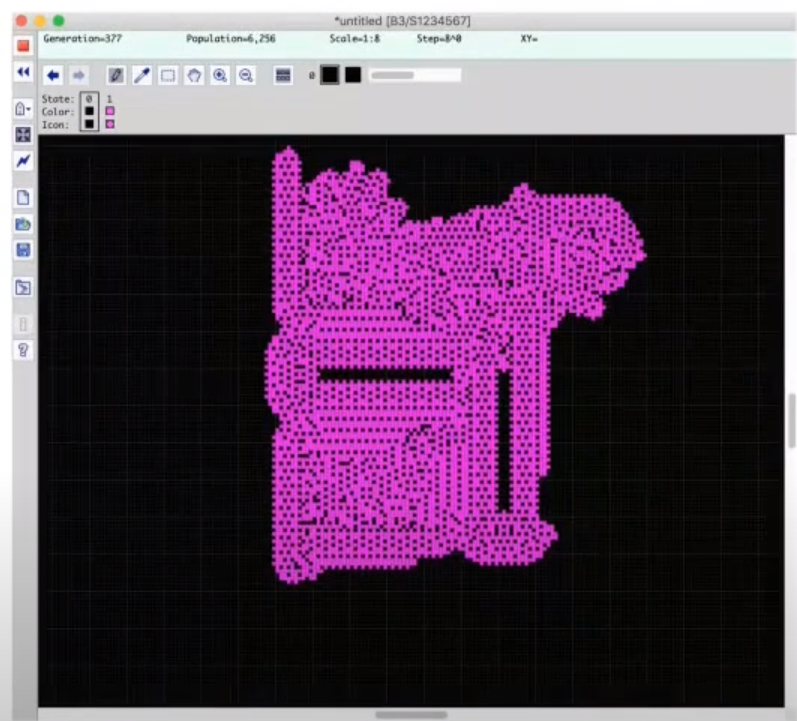
\includegraphics[width=0.4\textwidth]{lifesinmuerte.png}
\end{figure}
\begin{figure}[h!]
    \centering
    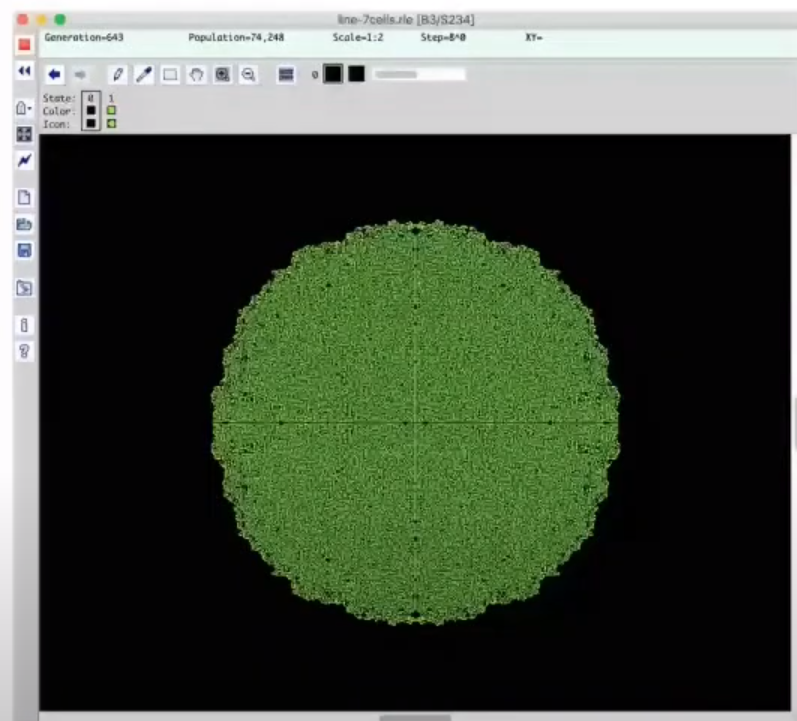
\includegraphics[width=0.4\textwidth]{vidacirculo.png}
\end{figure}
\begin{figure}[h!]
    \centering
    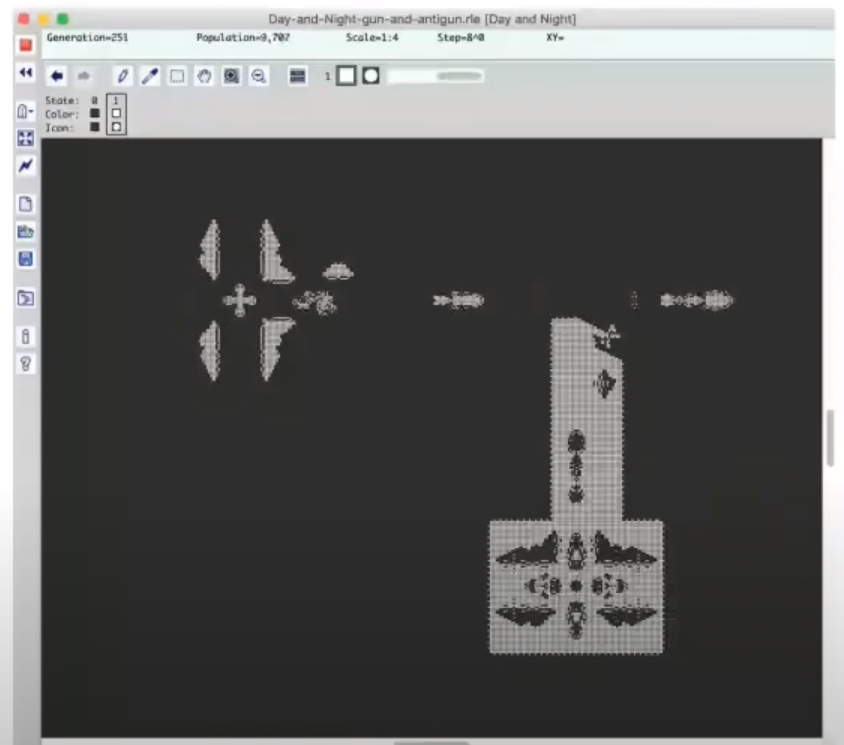
\includegraphics[width=0.4\textwidth]{dianoche.png}
\end{figure}
\newpage
Las reglas derivadas de life se pueden clasificar en 
\begin{itemize}
    \item Estables
    \item Periodicamente estables
    \item Casi-periodicamente estables
    \item Inestables
    \item Orbitadores
\end{itemize}

La regla B2/S2345 permite la implementación de circuitos lógicos. Historicamente, algunos autómatas celulares se basan en gliders, presencia o ausencia de patrones. El estudio actual se basa en el analisis de señales como un tipo de propagación de ondas donde paquetes de celulas viajan en canales en pelea de espacio.


    \begin{figure}[h!]
        \centering
        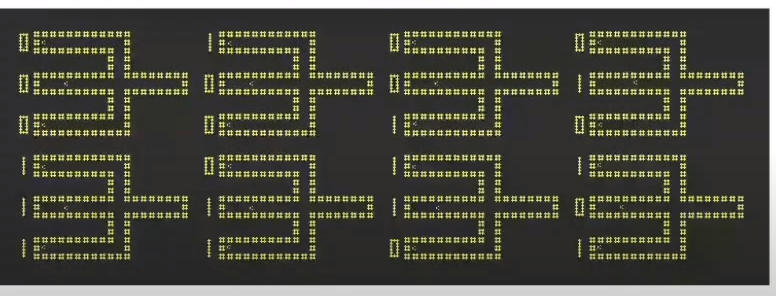
\includegraphics[width=0.5\textwidth]{b2.png}
    \end{figure}
    \bibliographystyle{apacite}
    \begin{thebibliography}{1}
        \bibitem[1]{c0}Cellular Automata India. Day 2, Session 2: "Notes about the Game of Life and some Life-like rules" by Prof. Genaro Martinez. Recuperado 8 de sept de 2022, de \url{https://www.youtube.com/watch?v=WqKkmfOt9Ww}

    \end{thebibliography}
    
\end{document}